\documentclass[compress]{beamer}
\usepackage{beamerthemeproyxetex}


%\useoutertheme[footline=authorinstitutetitle]{miniframes}
%\usecolortheme{whale}
%\usecolortheme{orchid}
%\useinnertheme{rounded}


\title{FoLiA: Format for Linguistic Annotation}
\author{Maarten van Gompel}
\date{01-02-2011}
\usepackage{graphicx}
\usepackage{listings}
\usepackage{color}
\lstset{% general command to set parameter(s)
basicstyle=\footnotesize,
keywordstyle=\color{black}\bfseries\underbar,
identifierstyle=\color{black}\bfseries\underbar,
stringstyle=\ttfamily,
}


\begin{document}

\begin{frame}
	\titlepage %\smallraccoon\ilkuvt
\end{frame}

\section{Introduction}

\begin{frame}{Introduction}

    \begin{block}{Annotation formats in the field}
        \begin{itemize}
            \item Many ad-hoc and old-style annotation formats (CGN, Tadpole column format) 
            \item Many theoretic and specialised annotation formats with limited scope
            \item OVerly rich document encoding formats (TEI)
            \item Many conversions needed
            \item De-facto-standard for various ILK projects: SoNaR/DCOI
        \end{itemize}
    \end{block}
    
    \begin{block}{Limits Tadpole/Frog columned format}
        \begin{itemize}
            \item Simplistic format, lacking expressiveness of XML
            \item Six/seven columns currently, covering full screen width
            \item Lacking even expressiveness to fully output Frog's data!
        \end{itemize}
    \end{block}

    \begin{block}{Limits of DCOI}
        \begin{itemize}
            \item Not expressive enough for many kinds of annotation (such as sense annotation, correction annotation)
            \item Can't encode annotators
            \item Can't encode alternatives
        \end{itemize}
    \end{block}

\end{frame}


\begin{frame}{Objectives}
    \begin{block}{Objectives}
        \textbf{Objectives: Expressability, Extensability, Uniformity}
        \begin{itemize}        
            \item One generalised rich common XML-based format, supporting almost all we do at ILK
            \item Uniform and consistent paradigm for annotations of various kinds
            \item Built from a bottom-up application-oriented perspective
            \item Not committing to any particular tagset or language            
            \item Encoding many different annotation aspects similtaneously in a single file
            \item Support for sense annotation (DutchSemCor)
            \item Support for complex corrections (Valkuil $+$ Ticcl)
            \item Support for NER (HITIME)
            \item Support in Frog for reading and writing this format            
            \item Founded on the DCOI format (our de-facto standard)
            \item Inter-operability with ISO Data Category Registry
            \item Unicode compliant
            \item Fully open-source
        \end{itemize}        
    \end{block}
\end{frame}

\begin{frame}{Annotations}
    \begin{block}{Supported Annotations}
        FoLiA supports the following linguistic annotations:
        \begin{itemize}
            \item Part-of-Speech tags (with features)
            \item Lemmatisation
            \item Spelling corrections on both a tokenised as well as an untokenised level.
            \item Domain tagging
            \item Semantic sense annotation (to be used in DutchSemCor)
            \item Named Entities / Multi-word units
            \item Syntactic Parses
            \item Dependency Relations
            \item Chunking
            \item Corrections
        \end{itemize}
    
        More to be added when needed (in collaboration with partners)

    \end{block}
\end{frame}

\section{Format}

\begin{frame}[fragile]
\frametitle{Format: Overall skeleton}
\begin{lstlisting}[language=xml]
<?xml version="1.0" encoding="utf-8"?>
<FoLiA xmlns="http://ilk.uvt.nl/FoLiA"
  xmlns:xsi="http://www.w3.org/2001/XMLSchema-instance"
  xml:id="example">
  <metadata>    
    <annotations>
      ...
    </annotations>    
    <!-- (Here IMDI or CMDI metadata can be inserted) -->
  </metadata>
  <text xml:id="example.text">
     ...
  </text>
</FoLiA>  
\end{lstlisting}
\end{frame}

\begin{frame}
    \begin{block}{Characteristic of overall format}
      \begin{enumerate}
        \item Unique identifier for document as a whole
        \item Metadata 
        \begin{itemize}
            \item Annotations - Declaration of all used annotations
            \item May hold IMDI or CMDI metadata
        \end{itemize}
        \item Text        
      \end{enumerate}
    \end{block}
\end{frame}



\begin{frame}[fragile]
\frametitle{Format: Basic structure}
\begin{lstlisting}[language=xml]
<p xml:id="TEST.p.1">
    <t>This is a test. It has two sentences.</t>
    <s xml:id="TEST.p.1.s.1">        
        <t>This is a test.</t>
        <w xml:id="TEST.p.1.s.1.w.1"><t>This</t></w>
        <w xml:id="TEST.p.1.s.1.w.2"><t>is</t></w>
        ..
    </s><s xml:id="TEST.p.1.s.2">...</s>                
</p>                
\end{lstlisting}
    
\end{frame}

\begin{frame}
    \begin{block}{Characteristics of basic structure}
      \begin{enumerate}
        \item \textbf{Structure Elements}: Paragraphs, Sentences, Words/Tokens  
        \item More: Division, Head, List, ListItem, Figure, Gap...
        \item Unique identifiers (DCOI style by convention)
        \item Text element (t) holds actual text.
      \end{enumerate}
    \end{block}
\end{frame}
        
        

\section{Paradigm}

\begin{frame}
    \begin{block}{Paradigm: Amnotation Categories}
            
        
        Three categories of annotation:    
        \begin{itemize}            
            \item \textbf{Structure Annotation} - Elements denoting document structure (division, paragraphs, lists, etc)
            \item \textbf{Token Annotation} - Linguistic Annotations pertaining to a single token (inline annotation)
            \item \textbf{Span Annotation} - Linguistic Annotations spanning over multiple tokens (standoff annotation)
        \end{itemize}
            
    \end{block}
\end{frame}

        
\begin{frame}
    \begin{block}{Paradigm: Common Attributes}
            
        FoLiA Attributes common to the paradigm.
        \begin{itemize}
            \item \textbf{ID} - A unique ID for the element
            \item \textbf{Set} - A particular tagset
            \item \textbf{Class} - A class in such a set
            \item \textbf{Annotator} - An open identifier for the user/system who provided the annotation
            \item \textbf{Annotator type} - ``auto'' or ''manual''
            \item \textbf{Confidence} - A confidence value between one and zero.
            \item \textbf{N} - A sequential number (for numbered divisions/sections, list items, etc)            
        \end{itemize}
            
    \end{block}
\end{frame}


\begin{frame}
        \frametitle{Paradigm: Schematic}
        \begin{center}
        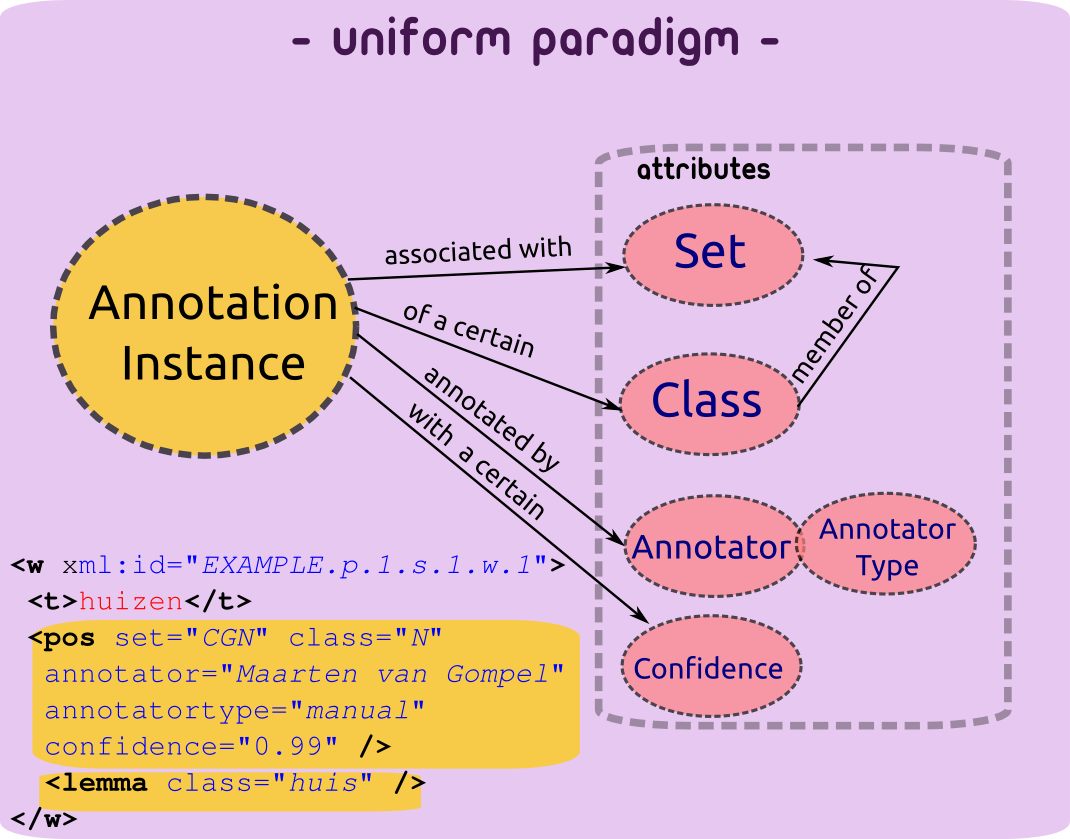
\includegraphics[width=90.0mm]{paradigm.png}
        \end{center}
\end{frame}


\section{Token Annotation}

\begin{frame}[fragile]
    \begin{block}{Token Annotation}
        Token annotation occurs within the scope of a word/token (\emph{w}) element.
    \end{block}
    \begin{example}
       PoS and Lemma Annotation:
\begin{lstlisting}[language=xml]
<w xml:id="example.p.1.s.1.w.2">
    <t>boot</t>
    <pos set="brown" class="n" />
    <lemma set="english-lemmas" class="boot" />
</w>                         
\end{lstlisting}        
    \end{example}
\end{frame}




\end{document}
